\documentclass[fontsize=12pt]{scrartcl}
\usepackage[ngerman]{babel}
\usepackage[utf8]{inputenc}
%\usepackage[latin1]{inputenc}
\usepackage{amsmath}
\usepackage{amstext}
\usepackage{amssymb}
\usepackage{stmaryrd}
\usepackage{verbatim}
\usepackage{mathrsfs}
\usepackage{extarrows}
\usepackage[arrow, matrix, curve]{xy}
\usepackage[centering,includeheadfoot,margin=2cm]{geometry}
\usepackage{gensymb}
\usepackage{graphicx}
\usepackage{framed}
\usepackage{xcolor}
\usepackage{float}
\usepackage{graphicx} 
\usepackage{sidecap}
\usepackage{blindtext,wrapfig}
\usepackage{epstopdf}
\usepackage{import}
\usepackage{fancyhdr}
\usepackage{fancybox}
\usepackage{paralist}
\usepackage{graphicx}
\usepackage{caption}
\usepackage{subcaption}
\renewcommand{\l}{\left\vert}
\renewcommand{\r}{\right\vert}
\newcommand{\define}{\ensuremath{\mathrel{\mathop:}=}} % hübscheres :=, da = zentriert wird relativ zu :
\newcommand{\enifed}{\ensuremath{=\mathrel{\mathop:}}} % hübscheres =:, da = zentriert wird relativ zu :
\DeclareGraphicsRule{.tif}{png}{.png}{`convert #1 `basename #1 .tif`.png} 
\pagestyle{fancy}
\fancyhf{}
\fancyhead[R]{Physikalisches Praktikum 1}
\fancyhead[L]{Robin Frank, Gentian Rrafshi}
\fancyfoot[R]{\thepage}
\fancyfoot[L]{\today}
\parindent 0pt
\parskip 12pt
\begin{document}

\begin{minipage}{0.9\textwidth}
\begin{center}\large
\title{ M30a – Erzwungene Schwingung und Resonanz \\
		~\\
		~\\
		Assistent: Simon Zimmermann \\
		Datum Versuchsdurchführung: \\
		10.07.2015}

\author{bearbeitet von\\
		Robin Frank Matrnr. 2887072 \\
		Gentian Rrafshi Matrnr. 2721617 }
\date{\today}

\maketitle

\end{center}
\end{minipage}

\newpage

\tableofcontents

\newpage
\noindent

\section{ Versuchsziel}

Bestimmung der Eigenfrequenz im gedämpften und ungedämpften Fall eine Schwingung und des logarithmischen Degrements.

\section{ Grundlagen}

Grundlage des Versuchs ist die sogenannte harmonische Schwingung. Eine Schwingung ist genau dann harmonische, wenn ihre zweite zeitliche Ableitung der gesuchten Funktion linear abhängig ist zu gesuchten Funktion. In Formeln heißt dies:
\begin{equation*}
\ddot{x}(t) = a\cdot x(t)
\end{equation*}
Bei einer mechanischen Schwingung lautet die DGL explizit:
\begin{equation*}
m\cdot \ddot{x}(t) - D\cdot x(t) = 0
\end{equation*}
Wobei hier m die Masse der Feder und D die Federkonstante ist.
Wie jede DGL n-ter Ordnung lässt sich auch diese DGL in eine DGL erster Ordnung zurückführen durch:
\begin{align*}
\dot{\vec{x}}(t)
\define
{\begin{pmatrix}
 \dot{x}(t)  \\
 \ddot{x}(t)  \\
\end{pmatrix}}
=
\begin{pmatrix}
0 & 1  \\
-\frac{m}{D} & 0  \\
\end{pmatrix}
\cdot 
\begin{pmatrix}
{x}(t)  \\
 \dot{x}(t)  \\
\end{pmatrix}
\enifed
\begin{pmatrix}
0 & 1  \\
-\frac{m}{D} & 0  \\
\end{pmatrix}
\cdot
\vec{x}(t)
\end{align*}
Die Lösung dieser DGL ist dann einfach
\begin{align*}
\vec{x}(t)
=
\begin{pmatrix}
c_1 \cos(\sqrt{\frac{m}{D}}t) &c_2 \sqrt{\frac{D}{m}} \sin(\sqrt{\frac{m}{D}}t)  \\
-c_1 \sqrt{\frac{D}{m}} \sin(\sqrt{\frac{m}{D}}t) &c_2 \cos(\sqrt{\frac{m}{D}}t) \\
\end{pmatrix}
\end{align*}
Die gesuchte Lösung unserer harmonischen Schwingung ist dann gegeben durch:
\begin{align*}
x(t) &=
e^{\intercal}_1 \vec{x}(t)
=
\begin{pmatrix}
1 &0  \\
\end{pmatrix}
\cdot
\begin{pmatrix}
c_1 \cos(\sqrt{\frac{m}{D}}t) &c_2 \sqrt{\frac{D}{m}} \sin(\sqrt{\frac{m}{D}}t)  \\
-c_1 \sqrt{\frac{D}{m}} \sin(\sqrt{\frac{m}{D}}t) &c_2 \cos(\sqrt{\frac{m}{D}}t) \\
\end{pmatrix}\\
~\\
&=c_1 \cos(\sqrt{\frac{m}{D}}t) +c_2 \sqrt{\frac{D}{m}} \sin(\sqrt{\frac{m}{D}}t) \\
&=\tilde{c_1} \cos(\sqrt{\frac{m}{D}}t)  + \tilde{c_2}\sin(\sqrt{\frac{m}{D}}t) \\
&=\tilde{c_1} \cos(\omega \cdot t)  + \tilde{c_2}\sin(\omega \cdot t) 
\end{align*}
Hierbei ist $\omega$ die sogenannte die Kreisfrequenz ist und $\tilde{c_1}, \tilde{c_2}$ abhängig von dem Anfangswertwertproblem ist.
\newpage
Für das Anfangswertproblem $x(0)=x_a$ erhalten wir 
\begin{align*}
x(t)=x_a \cdot cos(\omega \cdot t)
\end{align*}
und für $x(0)=0$ erhalten wir
\begin{align*}
x(t)=x_a \cdot sin(\omega \cdot t)
\end{align*}
wobei hier $x_a$ die Amplitude der Schwingung ist.

\section{Versuchsaufbau und Durchführung}

\subsection{Versuchsaufbau}
\begin{figure}[H]
\centering
\vspace{-10pt}
                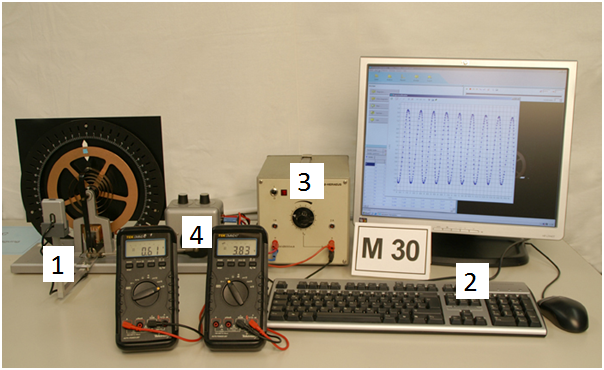
\includegraphics[width=0.7\textwidth]{Graphik/Versuch}
                \caption{Versuchsskizze$^{\cite{A}}$}
\end{figure}
\vspace{-10pt}
Die Grundlage der in diesem Versuch durchgeführten Messreihen stellt ein Drehpendel dar. Mithilfe diesem Drehpendels werden die Größen: Winkel $\Psi$ und das Drehmoment $M_i$ betrachtet.\par

Das Grundsystem wird wie folgt aufgebaut:\\
Das Drehpendel nach Pohl besteht aus einem kugelgelagertem Schwungrad, welches durch eine Spiralfederzentrisch in der Mitte mit einer Achse verbunden ist. Am äußeren Ende der Spiralfeder wird mit einem Erregergestänge verbunden, welches an einer exzentrischen Schwungscheibe am Elektromotor befestigt ist. 
Das Drehpendel kann durch eine Wirbelstrombremse gedämpft werden. Diese ist über ein Strommessgerät mit der Stromquelle verbunden. 
Der Elektromotor ist mit der Stromquelle verbunden, die Drehzahl kann beliebig eingestellt werden. (Mittels grob- und feinem Drehzahlregler).
Mittels einer Kamera kann über den PC die Pendelbewegung aufgezeichnet und mittels geeigneter Software ausgewertet werden. \par

Folgende Komponenten werden in diesem Versuch verwendet: \\
Drehpendel nach Pohl (Kästchen 1); Strommessgerät (Kästchen 4), Elektromotor als Schwingungsgeber (Kästchen 3), PC-System zur grafischen Analyse (Kästchen 2)

\subsection{Versuchsdurchführung}

\subsubsection{Ermittlung der Eigenfrequenz}

Für die Ermittlung der Eigenfrequenz für die ungedämpfte Schwingung wird nur das Drehpendel benötigt. Es wird jeweils die Schwingungsdauer von 10 Schwingungen gemessen bei Auslenkungen $<90^{\circ}$. Es sind 5 Messungen durchzuführen, jeweils mit unterschiedlicher Startauslenkung.\par

Für den gedämpften Fall wird nun die Wirbelstrombremse zur Hilfe genommen, bei der Mittels Wirbelstromfeld das kugelgelagerte Kupferrad während den Schwingungen abgebremst wird. Auch hier sind wieder 5 Messungen von 10 Schwingungen bei jeweils unterschiedlicher Startauslenkung($>90^{\circ}$) und unterschiedlicher Magnetfeldstärke (Stromstärke der Wirbelstrombremse – 0,2 A und 0,4A) durchzuführen.	

\subsubsection{Bestimmung des logarithmischen Dekrements $\Lambda$ und der Abklingkonstanten $\delta$}

Mithilfe der Kamera, die auf das Federpendel gerichtet ist, werden die Schwingungen aufgezeichnet. Aufgezeichnet wird die gedämpfte Schwingung bei jeweils 0,2A und 0,4A für die Dauer von 10-15 Schwingungen. Hierfür wird die Software „CaptureFlux“ und das Kamerasystem „Philips SPC 1300NC“ verwendet, welches Rohdaten im AVI Format bei einer Auflösung von 320x240 liefert, verwendet. \par

Mittels der Analyse Software „ Measure Dynamics“ wird die X,Y Pendelbewertung automatisiert (mittels Farb- und Bewegungserkennung) ausgewertet und als CSV Datei abgespeichert. (Siehe Auswertung). \par

Mittels der X,Y – Positionen wird der Amplitudenauslenkwinkel berechnet. Die Werte werden in einer zusätzlichen Spalte gespeichert.
Jetzt lässt sich der Verlauf der Schwingungen grafisch darstellen und das Dekrement ablesen, bzw. kann über das Steigungsdreieck berechnet werden

\subsubsection{Qualitativer Vergleich zwischen gedämpften und ungedämpften Verhalten}

Es ist eine ungedämpfte Schwingung aufzuzeichnen, und die X,Y Koordinaten sind wieder abzuspeichern. Daraufhin soll ein $\Psi(t)$ Diagramm erstellt werden. Die Ergebnisse sind mit den Messwerten aus Messreihe 3.2.2 zu Vergleichen.

\newpage

\subsubsection{Aufzeichnung der Resonanzkurve und Phasenverschiebung}

Für die bereits oben genannten Stromstärken (0,2\,A und 0,4\,A) wird die Resonanzkurve von Amplitude und Phasenverschiebung, in Abhängigkeit der Winkelgeschwindigkeit ermittelt. \par

Die Erregerfrequenz des Elektromotors kann mithilfe eines Groben und eines feinen Drehreglers eingestellt werden. Es sind 10 Messungen vorzunehmen, 5 über und 5 unter der Eigenfrequenz des Schwingsystems. Die Eigenfrequenz lässt sich z.B. aus der ersten Messreihe ermitteln. (Genaueres siehe im Punkt Auswertung der Daten). \par

Ist die Erregerfrequenz des Elektromotors eingestellt wird zur Aufnahme der Messung die Amplitude abgelesen. (Einschwingvorgänge sind abzuwarten, daher ist es sinnvoller bei der Messung mit dem größeren Bremsmoment, sprich 0,4A zu beginnen und dann jeweils umzustellen.) \par

Aus allen aufgezeichneten Werten lässt sich mithilfe Gl. (M30-8) und (M30-11) bei gegebener Phasenverschiebung die Resonanzkurve ermitteln.
\newpage
\section{Formeln}

\subsection{Formel für die Eigenfrequenz}

\begin{equation}
\omega_0=2\cdot \pi \cdot \frac{1}{T}
\label{T}
\end{equation}

$T$ [s]: Periodendauer;
$\omega$ [$\frac{1}{\text{s}}$]: Eigenfrequenz;

\subsection{Formel des Dekrements $\Lambda$}

\begin{equation}
\Lambda = \frac{1}{k} \cdot \ln(\frac{\Psi_k}{\Psi_{k+n}})
\label{Lambda}
\end{equation}

$\Lambda$: logarithmisches Dekrement;
$\Psi_k$ [$^{\circ}$]: k-tes Maximum;

\subsection{Formel der Abklingkonstante $\delta$}

\begin{equation}
\delta  = \frac{\Lambda}{T}
\label{delta}
\end{equation}

$\Lambda$: logarithmisches Dekrement;
$T$ [s]: Periodendauer;
$\delta$ [$\frac{1}{\text{s}}$]: Abklingkonstante;

\subsection{Formel für die Phasenverschiebung}
\begin{equation}
\tan(\phi)=  \frac{2\Lambda_{1/2}\omega}{T_{1/2}(w_0^2-w^2)}=\frac{2\Lambda_{1/2}\omega_{1/2}}{\pi(w_0^2-w^2)}\omega
\label{tan}
\end{equation}
$T_{1/2}$ [s]: Periodendauer schwach bzw. stark gedämpften Schwingung;
$\omega_{1/2}$ [$\frac{1}{\text{s}}$]: jeweilige Kreisfrequenzen;
$\Lambda_{1/2}$: jeweilige Dekremente;

\newpage

\section{ Messwerte}
\begin{figure}[H]
\centering
\caption{Messwerte ungedämpfte Schwingung}
\begin{tabular}{|c|c|} \hline
Auslenkung $\varphi$ 	[$^{\circ}$] & Zeit $T$ [s]\\ \hline
75	&18,58 \\ \hline
60	&18,59\\ \hline
45	&18,57\\ \hline
30	&18,61\\ \hline
15	&18,55\\ \hline
\end{tabular}					
\end{figure}

\begin{figure}[H]
\centering
\begin{minipage}{0.45\textwidth}
\centering
\caption{gedämpfte Schwingung;\\ I=0,2\,A}
\begin{tabular}{|c|c|} \hline
Auslenkung $\varphi$ 	[$^{\circ}$] & Zeit $T$ [s]\\ \hline
150	&18,55\\ \hline
135	&18,54\\ \hline
120	&18,49\\ \hline
105	&18,56\\ \hline
97,5	&18,56\\ \hline
\end{tabular}	
\end{minipage}	
\begin{minipage}{0.45\textwidth}
\centering
\caption{gedämpfte Schwingung;\\ I=0,4\,A}
\begin{tabular}{|c|c|} \hline
Auslenkung $\varphi$ 	[$^{\circ}$] & Zeit $T$ [s]\\ \hline
150	&18,71\\ \hline
135	&18,68\\ \hline
120	&18,71\\ \hline
105	&18,67\\ \hline
97,5	&18,70\\ \hline
\end{tabular}	
\end{minipage}
\end{figure}
\begin{figure}[H]
\caption{Messwerte Phasenverschiebung}
\centering
\begin{tabular}{|c|c|c|} \hline
&I=0,2\,A&I=0,4\,A\\ \hline
Frequenz $f$ [Hz] & Auslenkung $\varphi$ 	[$^{\circ}$] &Auslenkung $\varphi$ 	[$^{\circ}$] \\ \hline
0,20	&4,50	&4,50\\ \hline
0,30	&6,00	&6,00\\ \hline
0,35	&6,75	&6,75\\ \hline
0,40	&8,25	&8,25\\ \hline
0,45	&12,75	&12,75\\ \hline
0,50	&25,50	&22,50\\ \hline
0,52	&67,50	&40,50\\ \hline
0,54	&105,00	&49,50\\ \hline
0,56	&37,50	&33,00\\ \hline
0,58	&28,50	&15,00\\ \hline
0,60	&13,50	&13,50\\ \hline
0,65	&6,00	&6,00\\ \hline
0,70	&5,25	&5,25\\ \hline
\end{tabular} \\
\end{figure}

\newpage

\section{ Auswertung}

\subsection{Ermittelung der Eigenfrequenzen}

Hierfür benötigen wir zuerst die Periodendauer des Schwingungen. Durch mitteln unserer Zeitmessungen erhalten wir die Periodendauer über 10 Perioden. Wir erhalten also die Gleichung:
\begin{align*}
\bar{T}= \frac{\sum\limits^5_{k=1} t_k}{5 \cdot 10}
\end{align*}
Beispielhaft wird hier an der ungedämpften Schwingung die Periodendauer berechnet:
\begin{align*}
\bar{T}= \frac{\sum\limits^3_{k=1} t_k}{3 \cdot 10} =\frac{ t_1+t_2+t_3+t_4+t_5}{50} =\frac{ 18,58\,\text{s}+18,59\,\text{s}+18,57\,\text{s}+18,61\,\text{s}+18,55\,\text{s}}{50}=1,85\,\text{s}
\end{align*}
Dann lässt sich durch Formel (\ref{T}) die Eigenfrequenz berechnen. Auch hier eine Beispielrechnung:
\begin{align*}
\omega_0=2\cdot \pi \cdot \frac{1}{1,85\,\text{s}} =3,38\,\frac{1}{\,\text{s}}
\end{align*}
Die restlichen Werte sind in der nachfolgenden Tabelle ablesbar:
\begin{figure}[H]
\caption{Ergebnisse Eigenfrequenz}
\centering
\begin{tabular}{c|c|c} \hline
Art Schwingung $f$ [Hz] & Periodendauer $\bar{T} $	[s] & Eigenfrequenz $\omega_0\,[\,\frac{1}{\,\text{s}}]$ \\ \hline
ungedämpft &1,86	&3,38 \\ \hline
gedämpft I=0,2\,A&1,85&	3,38 \\ \hline
gedämpft I=0,4\,A&1,87&	3,36 \\
\end{tabular} \\
\end{figure}
Unsere Ergebnisse zeigen nur eine kleine Änderung in der Eigenfrequenz durch die Dämpfung an.
\newpage
\subsection{Logarithmisches Dekrement und die Abklingkonstante}

Wir erhalten folgende Graphen:
\begin{figure}[H]
\centering
\vspace{-10pt}
                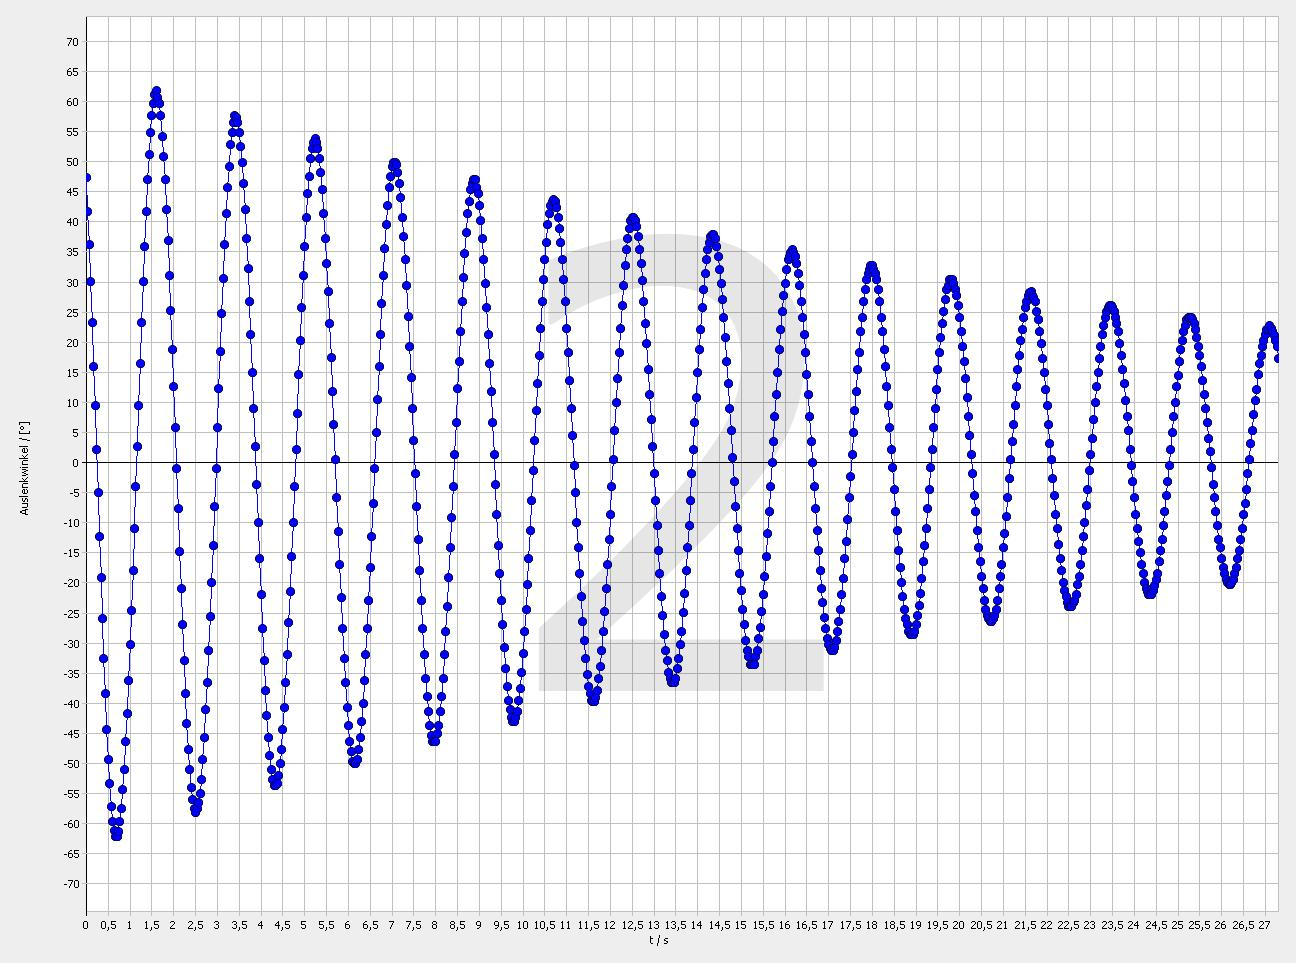
\includegraphics[width=0.7\textwidth]{Graphik/RobinGenti0,2}
                \caption{schwach gedämpfte Schwingung}
                \label{7}
\end{figure}
\vspace{-10pt}
\begin{figure}[H]
\centering
\vspace{-10pt}
                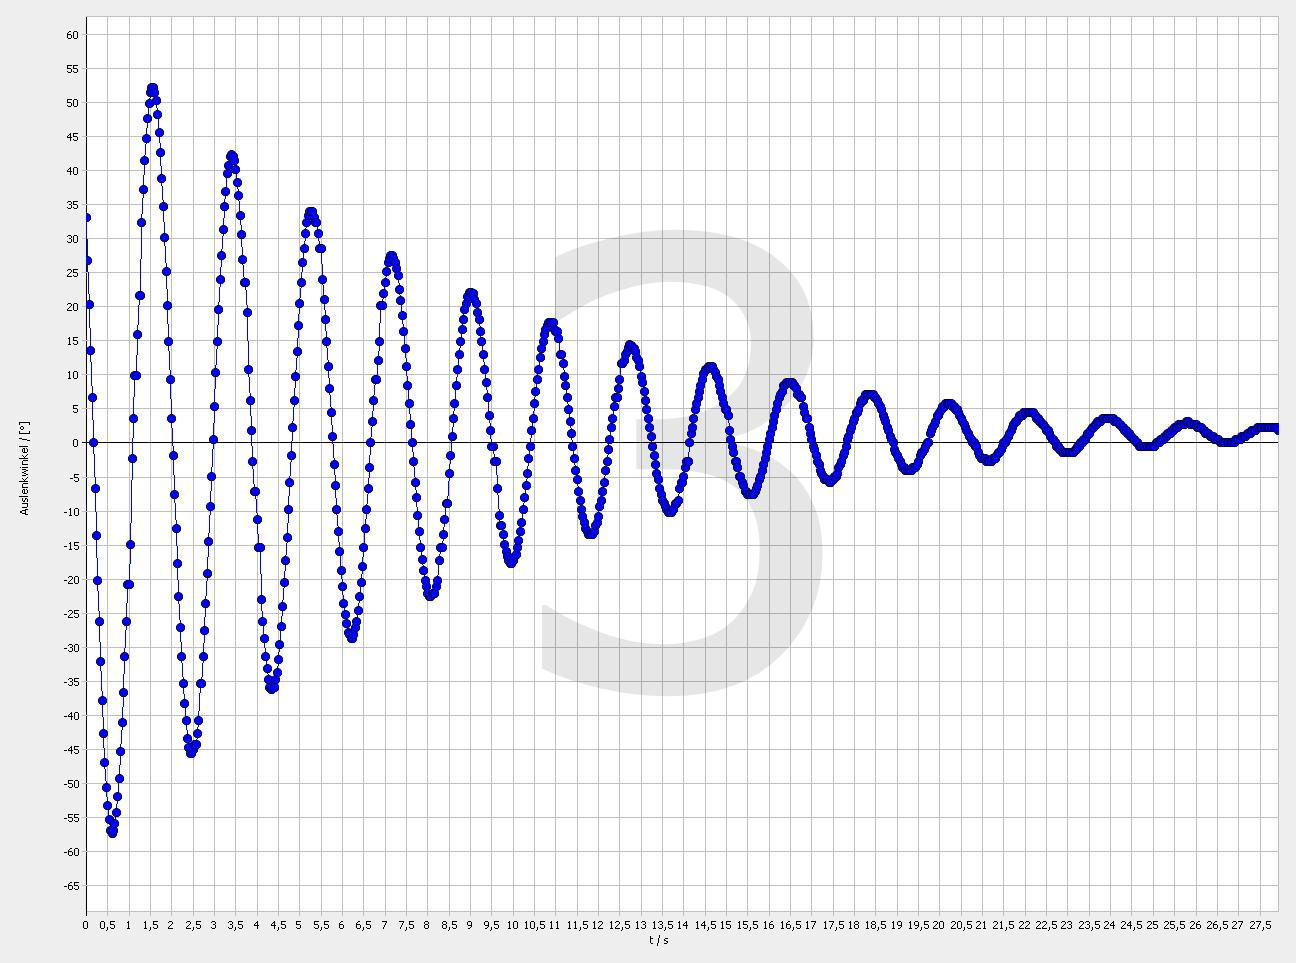
\includegraphics[width=0.7\textwidth]{Graphik/RobinGenti0,4}
                \caption{stark gedämpfte Schwingung}
                \label{8}
\end{figure}
\vspace{-10pt}
\newpage
Mit denen wir das logarithmische Dekrement errechnen sollten. Dafür nehmen wir Formel $(\ref{Lambda})$. Wir erhalten
\begin{align*}
\Lambda_{\text{schwach}} &= \frac{1}{k} \cdot \ln(\frac{\Psi_k}{\Psi_{k+n}})=\frac{1}{14-1} \cdot \ln(\frac{63^{\circ}}{30^{\circ}})=0,053 \\
~\\
\Lambda_{\text{stark}} &= \frac{1}{k} \cdot \ln(\frac{\Psi_k}{\Psi_{k+n}})=\frac{1}{14-1} \cdot \ln(\frac{53^{\circ}}{3^{\circ}})=0,205
\end{align*}
Durch entnehmen der Maxima und auftragen dieser über ihre Anzahl erhalten wir folgendes Diagramm, bei dem die y-Achse logarithmiert ist.
\begin{figure}[H]
\centering
\vspace{-10pt}
                \includegraphics[width=0.7\textwidth]{Graphik/dek}
                \caption{Amplituden-Periode-Diagramm}
                \label{9}
\end{figure}
\vspace{-10pt}
Durch Formel (\ref{delta}) erhalten wir nun recht einfach die Abklingkonstanten $\delta$.

\begin{align*}
\delta_{\text{schwach}}  = \frac{\Lambda_{\text{schwach}}}{T_{\text{schwach}}}= \frac{0,053}{1,85\,\text{s}} = 0,03\,\frac{1}{\text{s}}\\
~\\
\delta_{\text{stark}} = \frac{\Lambda_{\text{stark}}}{T_{\text{stark}}} = \frac{0,205}{1,87\,\text{s}}=0,11\,\frac{1}{\text{s}}
\end{align*}

\subsection{Vergleich ungedämpfte und gedämpfte Schwingung}
\begin{figure}[H]
\centering
\vspace{-10pt}
                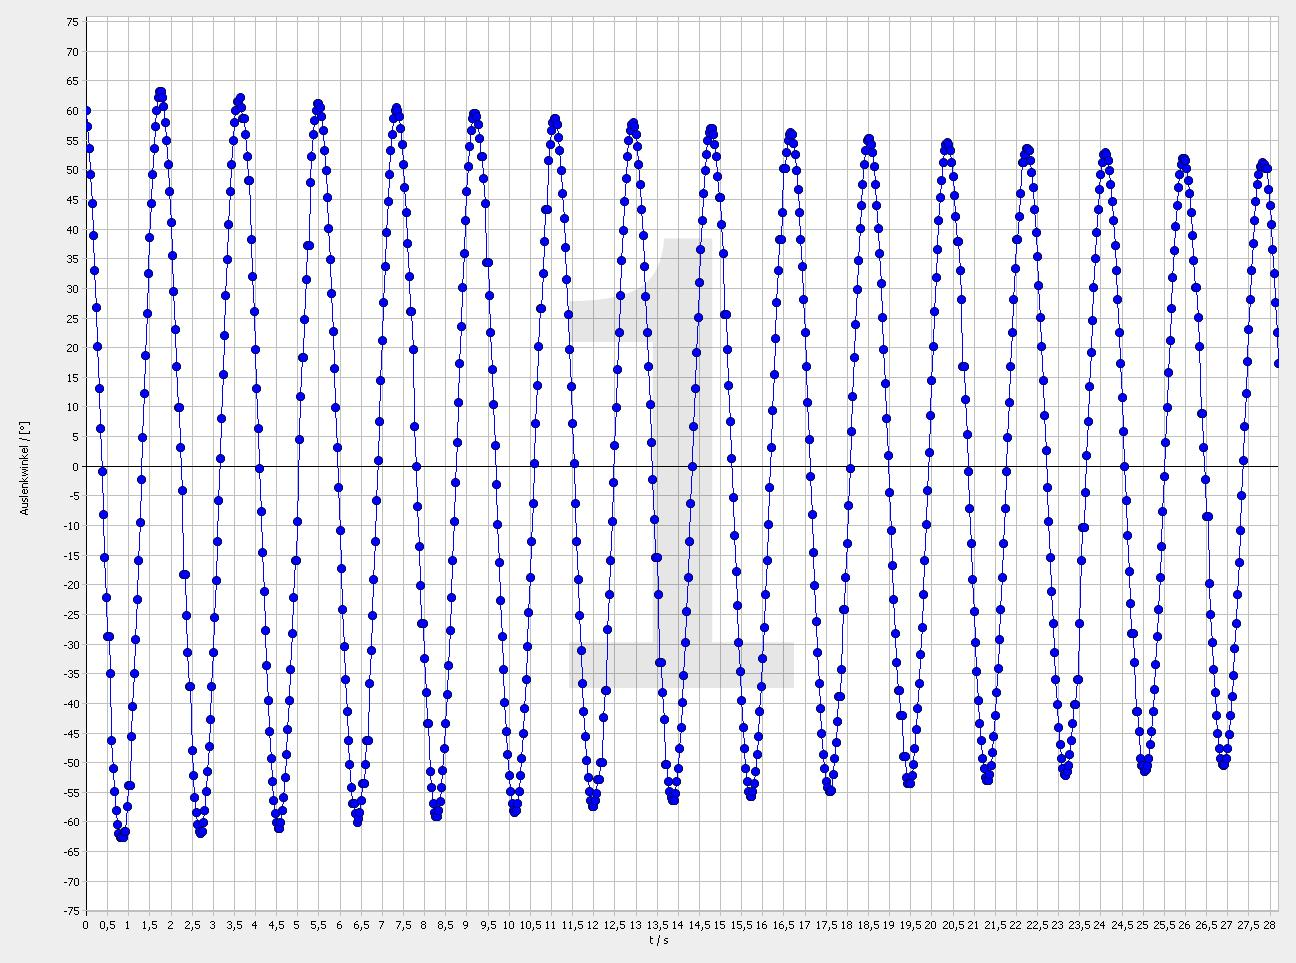
\includegraphics[width=0.7\textwidth]{Graphik/RobinGentiungedampft}
                \caption{stark gedämpfte Schwingung}
                \label{9}
\end{figure}
\vspace{-10pt}
Wie Abbildung (\ref{9}) zeigt, bleibt die Amplitude über den gesamten Zeitraum annähernd gleich und man sieht dazu in Abb.(\ref{7}) und Abb.(\ref{8}) wie die Amplitude schon nach einer Periode relativ stark abnimmt. Es ist auch ersichtlich, dass mit zunehmender Dämpfung auch die Amplituden schneller sinken.
\newpage
\subsection{Resonanzkurve}

Nun sollen wir die Resonanzkurven aufzeichnen. Dazu erhalten wir folgendes Diagramm:
\begin{figure}[H]
\centering
\vspace{-10pt}
                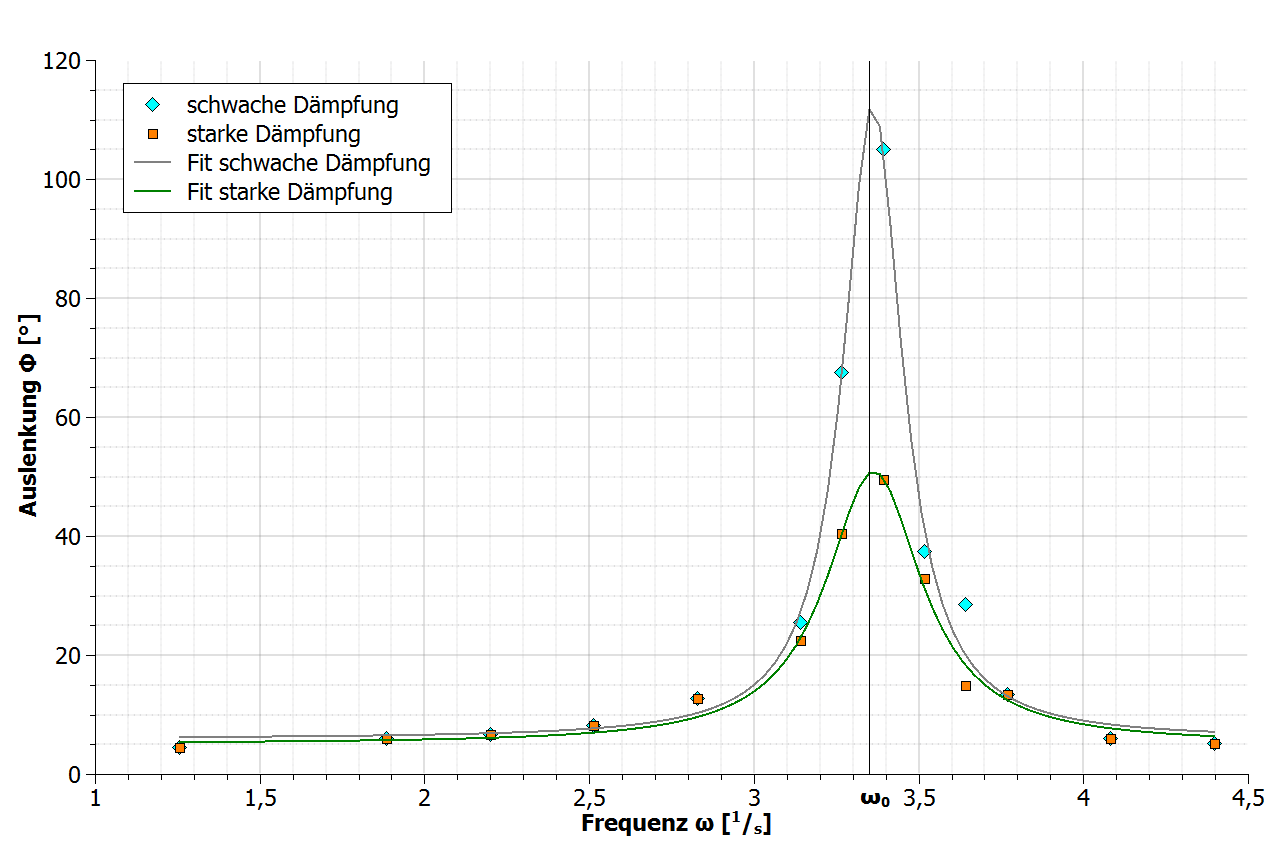
\includegraphics[width=0.7\textwidth]{Graphik/Resonanz}
                \caption{Resonanzkurven beider Dämpfungen}
\end{figure}
\vspace{-10pt}
Schön zu sehen ist, dass beide Kurven ihr Maximum an der Eigenfrequenz $\omega_0\approx3,38$ haben. Ersichtlich wird bei den Resonanzkurven auch die Einwirkung von höherer Dämpfung, welche sich durch Senken des Maximums wiedergibt.
\newpage
\subsection{Phasenverschiebung}

Dank Formel (\ref{tan}) wissen wir in etwa das Aussehen der Phasenverschiebung. Unsere Messwerte ergeben dazu folgendes Diagramm:
\begin{figure}[H]
\centering
\vspace{-10pt}
                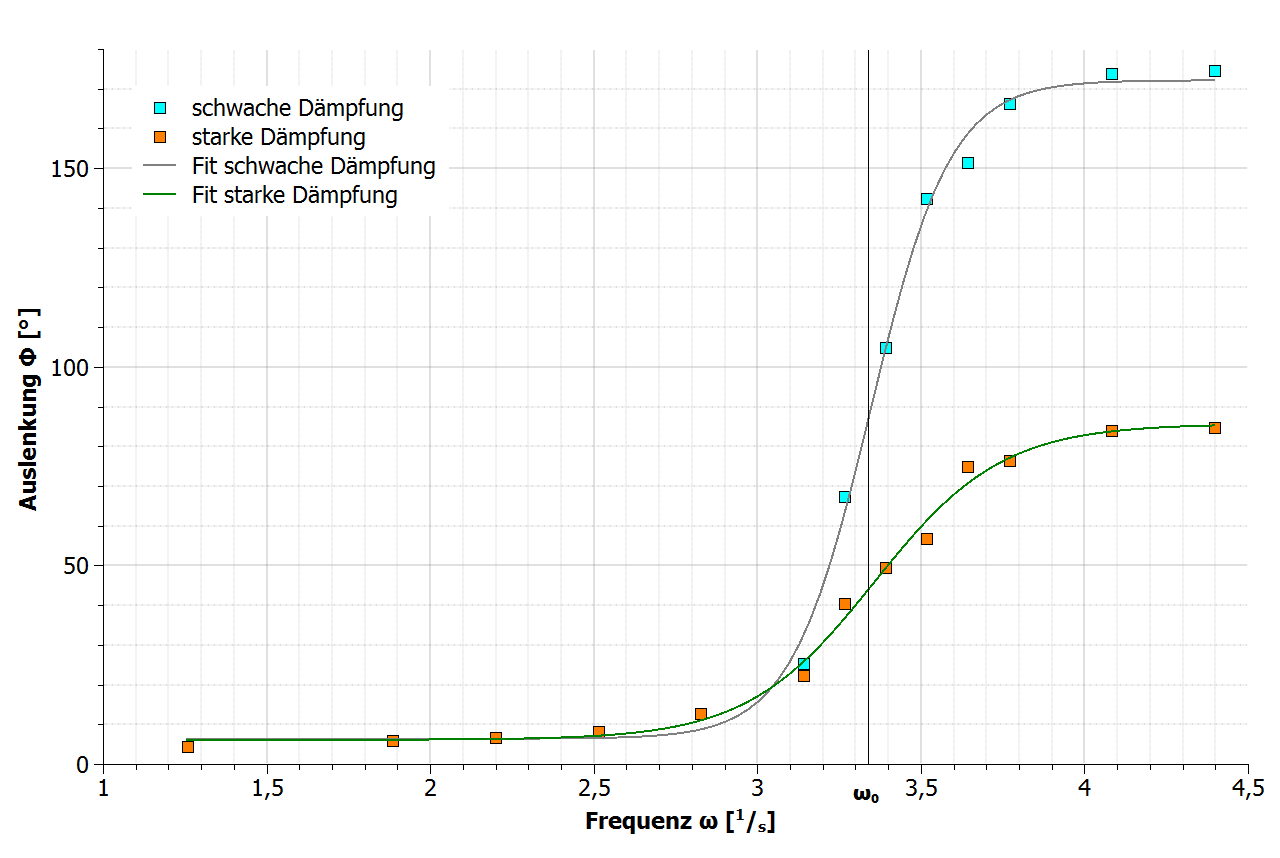
\includegraphics[width=0.7\textwidth]{Graphik/Phase}
                \caption{Phasenverschiebung beider Dämpfungen}
\end{figure}
\vspace{-10pt}
Einigermaßen ersichtlich ist hier, dass die Eigenfrequenz im Wendepunkt von unseren Fitkurven liegt. Auch hier erkennt man den Einfluss höherer Dämpfung, welches sich durch eine kleinere Auslenkung wiedergibt.

\newpage

\section{Fehlerrechnung}

\subsection{Fehler bei der Eigenfrequenzen}

Als Fehler dürfen wir $\Delta T=0,2$\,s annehmen Durch Formel (\ref{T}) erhalten wir, eine Beispiel wird gleich für den ungedämpften Fall mitgerechnet, damit:
\begin{align*}
\Delta \omega_0 &=\l\frac{\partial}{\partial T}\frac{2\pi}{T}\r \cdot \Delta T = \frac{2\pi}{T^2} \cdot \Delta T \\
&=2\cdot \pi \cdot \frac{1}{1,85^2\,\text{s}^2} \cdot  0,2\,\text{s} =0,36\,\frac{1}{\,\text{s}}
\end{align*}
Die restlichen Werte werden in der nachliegenden Tabelle dargestellt
\begin{figure}[H]
\caption{Ergebnisse Eigenfrequenz samt Fehler}
\centering
\begin{tabular}{c|c|c|c} \hline
Art Schwingung $f$ [Hz] & Periodendauer $\bar{T} $	[s] & Eigenfrequenz $\omega_0\,[\,\frac{1}{\,\text{s}}]$  & Fehler $\Delta \omega \,[\,\frac{1}{\,\text{s}}]$ \\ \hline
ungedämpft &1,86	&3,38&0,36 \\ \hline
gedämpft I=0,2\,A&1,85&	3,38 &0,36\\ \hline
gedämpft I=0,4\,A&1,87&	3,36 &0,36\\
\end{tabular} \\
\end{figure}

\subsection{Fehler logarithmisches Dekrement}

Es gilt ein Fehler von $\Delta \Psi=2^{\circ}$ und daher ergibt sich für das Dekrement:
\begin{align*}
\Delta \Lambda &= \l\frac{\partial}{\partial \Psi_{k}} \frac{1}{k} \cdot \ln(\frac{\Psi_k}{\Psi_{k+n}}) \r  \cdot \Delta\Psi_{k}+  \l\frac{\partial}{\partial \Psi_{k+n}} \frac{1}{k} \cdot \ln(\frac{\Psi_k}{\Psi_{k+n}}) \r\cdot \Delta\Psi_{k+n} \\
&=  \l \frac{1}{\Psi_k k}  \r  \cdot \Delta\Psi_{k}+  \l\frac{1}{\Psi_{k+n}k}\r \cdot \Delta\Psi_{k+n}
\end{align*}
Daraus ergibt sich nun:
\begin{align*}
\Delta \Lambda_{\text{schwach}} &=  \l \frac{1}{63^{\circ} 13}  \r  \cdot 2^{\circ}+  \l \frac{1}{30^{\circ}13}\r \cdot 2^{\circ}= 7,57 \cdot 10^{-3}\\
~\\
\Delta \Lambda_{\text{stark}} &=  \l \frac{1}{53^{\circ} 13}  \r  \cdot 2^{\circ}+  \l \frac{1}{3^{\circ}13}\r \cdot 2^{\circ}= 54,18 \cdot 10^{-3}
\end{align*}
Unsere Fehler ergeben Fehlerkurven in unserem Amplituden-Periode-Diagramm, welche wir im einem neuem Diagramm darstellen:
\begin{figure}[H]
\centering
\vspace{-10pt}
                \includegraphics[width=0.7\textwidth]{Graphik/fehler}
                \caption{Amplituden-Periode-Diagramm}
                \label{9}
\end{figure}
\vspace{-10pt}

\subsection{Fehler Abklingkonstante}

Aus $\Delta\Lambda$ und $\Delta T$ erhalten wir nun einen Fehler $\Delta\delta$ wie folgt
\begin{align*}
\Delta\delta &= \l\frac{\partial}{\partial  \Lambda } \frac{ \Lambda }{T} \r  \cdot \Delta \Lambda +  \l\frac{\partial}{\partial T} \frac{ \Lambda }{T} 
\r\cdot \Delta T \\
&= \l  \frac{ 1}{T} \r  \cdot \Delta \Lambda +  \l  \frac{ \Lambda }{T^2}  \r\cdot \Delta T \\
\end{align*}
Daraus ergibt sich nun:
\begin{align*}
\Delta\delta_{\text{schwach}}&= \l  \frac{ 1}{1,85\,\text{s}} \r  \cdot 7,75\cdot 10^{-3} +  \l  \frac{ 0,053}{(1,85\,\text{s})^2}  \r\cdot 0,2\,\text{s}=7,17\cdot 10^{-3}
 \\
~\\
\Delta\delta_{\text{schwach}} &= \l  \frac{ 1}{1,87\,\text{s}} \r  \cdot 54,18\cdot 10^{-3} +  \l  \frac{ 0,205}{(1,87\,\text{s})^2}  \r\cdot 0,2\,\text{s}=27,73\cdot 10^{-3}
 \\
\end{align*}

\newpage

\section{Zusammenfassung}

Unser erstes Ziel in diesem Versuch war es, die Eigenfrequenzen für unsere verschiedensten Systeme zu ermitteln. Wir bekamen folgende Werte heraus:
\begin{figure}[H]
\caption{Zusammenfassung Eigenfrequenz}
\centering
\begin{tabular}{c|c|c|c} \hline
Art Schwingung $f$ [Hz] & Periodendauer $\bar{T} $	[s] & Eigenfrequenz $\omega_0\,[\,\frac{1}{\,\text{s}}]$  & Fehler $\Delta \omega \,[\,\frac{1}{\,\text{s}}]$ \\ \hline
ungedämpft &1,86	&3,38&0,36 \\ \hline
gedämpft I=0,2\,A&1,85&	3,38 &0,36\\ \hline
gedämpft I=0,4\,A&1,87&	3,36 &0,36\\
\end{tabular} \\
\end{figure}

Dann sollten wir mit Hilfe dessen das logarithmische Dekrement und die Abklingkonstante von unseren gedämpften Systemen ermitteln. Es ergab sich bei uns, dass
\begin{align*}
\Lambda_{\text{schwach}} &= 0,053\pm  7,57 \cdot 10^{-3}\\
~\\
\Lambda_{\text{stark}} &=0,205\pm54,18 \cdot 10^{-3}
\end{align*}
für die logarithmischen Dekremente gilt und 
\begin{align*}
\delta_{\text{schwach}} &=  ( 0,03\pm7,17\cdot 10^{-3}) 			\,\frac{1}{\text{s}}\\
~\\
\delta_{\text{stark}} &= (0,11\pm27,73\cdot 10^{-3}	)	\,\frac{1}{\text{s}}
\end{align*}
Ergab sich für die Abklingkonstanten. \par

Weiter sahen wir in den Resonanzkurven, dass die Maximas an der Eigenfrequenz $\omega_0=3,38\frac{1}{\text{s}}$ waren und es sich dann in beide Richtung zur Null hin bewegt. Auch sah man den Einfluss einer höheren Dämpfung auf die Resonanzkurve, welche ein kleineres Maximum hervorruft. \par

In unserem Phasendiagramm sieht man ebenfalls welchen Einfluss einen höhere Dämpfung hat. Zum einen ist die Auslenkung kleiner, zum anderen steigen die Werte nicht so stark an in der näher der Eigenfrequenz, je größer die Dämpfung ist.
\newpage
\section{Literaturverzeichnis}

\renewcommand{\refname}{~}
\vspace{-30pt}
\begin{thebibliography}{xx}
   \bibitem[1]{1}  	   \textit{\glqq M30 Erzwungene Schwingung und Resonanz\grqq , in 	\\
   								http://www3.physik.uni-stuttgart.de/studium/praktika/ap/}, \\
   								abgerufen am  17.07.2015
   \bibitem[A]{A}  	Graphik aus \textit{\glqq M30 Erzwungene Schwingung und Resonanz\grqq , in 	\\
   								http://www3.physik.uni-stuttgart.de/studium/praktika/ap/}, \\
   								unter \textit{http://www3.physik.uni-stuttgart.de/studium/praktika/ap/pdf\_dateien/M30.pdf}; \\
   								abgerufen am  17.07.2015
\end{thebibliography}

\section{Anhang}

\end{document}